%%%%%%%%%%%%%%%%%%%%%%%%%%%%%%%%%%%%%%%%%%%%%%%%%%%%%%
% A Beamer template for Ritsumeikan University       %
% Author: Ming-Hao Xu (Xu Minghao)                   %
% Date:   April 2022.                                %
% LPPL Licensed.                                     %
%%%%%%%%%%%%%%%%%%%%%%%%%%%%%%%%%%%%%%%%%%%%%%%%%%%%%%

\documentclass{beamer}
\usepackage{hyperref}
\usepackage[T1]{fontenc}
\usepackage{caption}
\usepackage{bm}

% other packages
\usepackage{latexsym,amsmath,xcolor,multicol,booktabs,calligra}
\usepackage{graphicx,pstricks,listings,stackengine}
\usepackage{tikz}
\usetikzlibrary{calc,arrows}

\newcommand\blfootnote[1]{%
  \begingroup
  \renewcommand\thefootnote{}\footnote{#1}%
  \addtocounter{footnote}{-1}%
  \endgroup
}

% dummy text; remove it when working on this template
%\usepackage{lipsum}

\author{Nicolás Barrios Pizo}
\title{Simulaciones micromagnéticas en nanohilos ferromagnéticos de Co-Ni con anisotropía transversal}
\subtitle{Anteproyecto de Grado}
\institute{
    Departamento de Física \\
    Universidad del Valle
}
\date{11 de Junio del 2023}
\usepackage{Ritsumeikan}

% defs
\def\cmd#1{\texttt{\color{red}\footnotesize $\backslash$#1}}
\def\env#1{\texttt{\color{blue}\footnotesize #1}}
\definecolor{deepblue}{rgb}{0,0,0.5}
\definecolor{deepred}{rgb}{0.6,0,0}
\definecolor{deepgreen}{rgb}{0,0.5,0}
\definecolor{halfgray}{gray}{0.55}

\lstset{
    basicstyle=\ttfamily\small,
    keywordstyle=\bfseries\color{deepblue},
    emphstyle=\ttfamily\color{deepred},    % Custom highlighting style
    stringstyle=\color{deepgreen},
    numbers=left,
    numberstyle=\small\color{halfgray},
    rulesepcolor=\color{red!20!green!20!blue!20},
    frame=shadowbox,
}


\begin{document}

\begin{frame}
    \titlepage
    \begin{figure}[!htp]
        \centering
        
\includegraphics[keepaspectratio, scale=0.045]{../Main/logoUV_Oficial_Rojo.jpg}
    \end{figure}
\end{frame}

\begin{frame}
    \tableofcontents[sectionstyle=show,subsectionstyle=show/shaded/hide,subsubsectionstyle=show/shaded/hide]
\end{frame}

\section{Introducción}

\begin{frame}{Introducción}
    El \textbf{micromagnetismo} es una teoría continua que describe los procesos de magnetización en una escala tamaño significativa.
    
    \medskip
    
    \begin{figure}
        \centering
        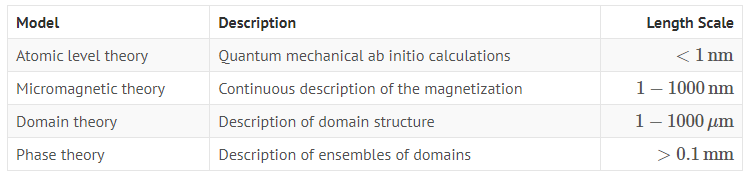
\includegraphics[scale=0.45]{pic/micromagnetism.png}
        \caption{Modelos establecidos para la descripción del ferromagnetismo en diferentes escalas de longitud.}
    \end{figure}
    
    \blfootnote{ {\tiny http:/micromagnetics.org/}}
    \blfootnote{ {\tiny Exl, L., Suess, D. y Schrefl, T. en Handbook of Magnetism and Magnetic Materials (eds. Coey, M. y Parkin, S.) 1-44 (Springer International Publishing, Cham, 2020).}}
\end{frame}

\begin{frame}
    \centering
    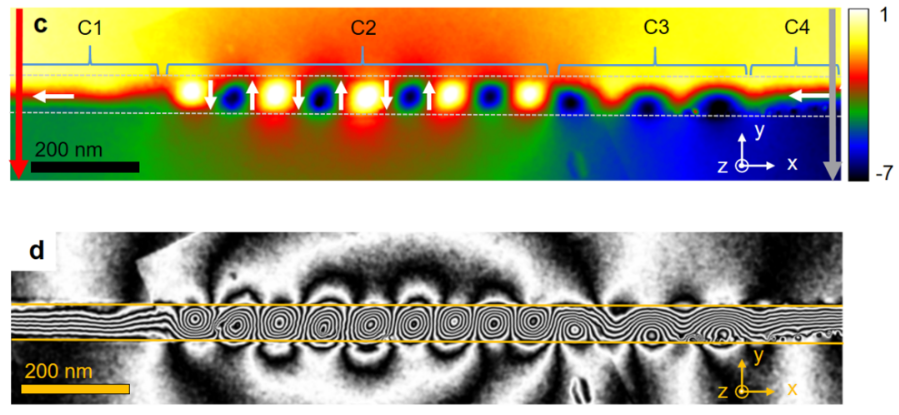
\includegraphics[scale=0.4]{pic/Vortex.png}
    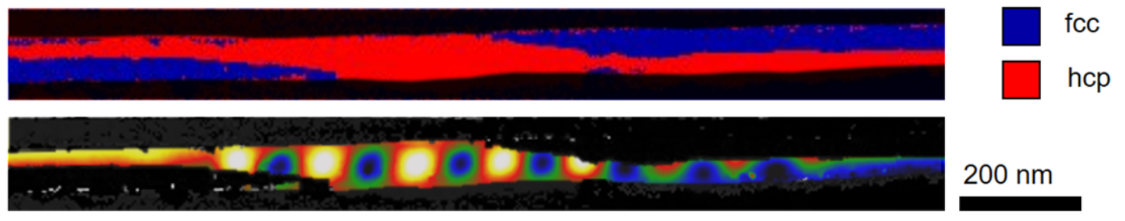
\includegraphics[scale=0.34]{pic/EstructuraCristalina.png}   
    \blfootnote{ {\tiny Andersen, I. M. et al. Exotic Transverse-Vortex Magnetic Configurations in CoNi Nanowires. ACS Nano 14, 1399-1405 (2020).}}
\end{frame}

\section{Marco Teórico}

\begin{frame}{Ecuaciones de Landau-Lifshitz y Gilbert}
    \begin{columns}
    % Column 1
    \begin{column}{0.5\textwidth}
    %La magnetización es la densidad de momentos magneticos, y como densidad que es, es una propiedad local del material. Asi que si analizamos la magnetización en una región infinitesimal, claramente la densidad de momentos magneticos no va a cambiar, y la magnitud de estos es constante y todos se alinean en dicha región. Por tanto, la magnetización solo gira.
        \footnotesize
        \textbf{Magnetización}
        \[ \bm{M}_s (\bm{r},T) = |M_s (T)| \sum_{n=1}^3 \gamma_n (\bm{r}) \hat{\bm{e}}_n \]
        
        \vspace{0.1cm}

        \textbf{Ecuaciones Diferenciales}
        \[ \frac{d \bm{M}_s}{dt} = \gamma_G (\bm{M}_s \times \bm{H}_{eff}) - \frac{\alpha_G}{M_s}(\bm{M}_s \times \frac{d \bm{M}_s}{dt})\]
        \[ \bm{H}_{eff} = - (1/J_s) \partial \phi_l / \partial \bm{m} ~~~ \wedge ~~~ \bm{m} = \bm{M}_s/M_s \]

        \vspace{0.2cm}
        
        \begin{itemize}
            \item $\gamma_G$: Constante giromagnética de los electrones.
            \item $\alpha_G$: Constante de amortiguamiento de Gilbert.
        \end{itemize}
    \end{column}
    % Column 2    
    \begin{column}{0.5\textwidth}
            \centering
            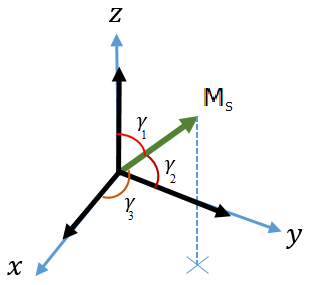
\includegraphics[width=3.5cm,height=3cm]{pic/CosenosDirectores.png}

            \vspace{0.5cm}
            
            \centering
            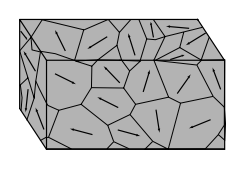
\includegraphics[width=3.5cm,height=3cm]{../Figuras/MagneticDomain.png}
    \end{column}
    \end{columns}
    \blfootnote{{\tiny Exl, L., Suess, D. y Schrefl, T. en Handbook of Magnetism and Magnetic Materials (eds. Coey, M. y Parkin, S.) 1-44 (Springer International Publishing, Cham, 2020).}}
\end{frame}

\begin{frame}{Energía libre de Gibbs}
        \begin{columns}
    % Column 1
    \begin{column}{0.5\textwidth}
    \footnotesize
        \textbf{Energía libre de Gibbs}
        \[ \phi'_l = U - T S - \sigma \cdot \epsilon - \bm{J}_s \cdot \bm{H}_{ext}\]
        \[ \phi_l = \int_v \phi'_l dV \]

        \vspace{0.7cm}
        
        \textbf{Densidad de energía interna}
        \[ U = \phi'_s + \phi'_K + \phi'_{ex} + \phi'_H + \phi'_{el}  \]
    \end{column}
    % Column 2    
    \begin{column}{0.5\textwidth}
    \scriptsize
        \begin{itemize}
            \item $S$: Entropía por unidad de volumen.
            \item $\sigma$: Tensor de estrés.
            \item $\epsilon$: Tensor de Tensión.
            \item $\bm{H}_{ext}$: Campo magnético externo.
            \item $T$: Temperatura.
        \end{itemize}

        \vspace{0.5cm}
        
        \begin{itemize}
            \item $\phi'_s$: Den. ener. dipolar.
            \item $\phi'_K$: Den. ener. anisotropía magnetocristalina.
            \item $\phi'_{ex}$:  Den. ener. intercambio.
            \item $\phi'_H$: Den. ener. Zeeman.
            \item $\phi'_{el}$: Den. ener. elástica.
        \end{itemize}
    \end{column}
    \end{columns}
    
    \vspace{0.3cm}

    \small
    En equilibrio termodinámico, la energía libre de Gibbs corresponde de a un mínimo ($\delta \phi_l = 0$). En donde $T$, $\sigma$ y $\bm{H}_{ext}$ son parámetros libres.

    \blfootnote{{\tiny Kronm uller, H. y Fahnle, M. Micromagnetism and the Microstructure of Ferromagnetic Solids (Cambridge University Press, 2003)}}
\end{frame}



\begin{frame}{Energía de Intercambio}
    \[ \mathcal{H}_{ex} = - 2 \sum_{i \neq j} J_{ij} \bm{S}_i \cdot \bm{S}_j ~~ \rightarrow ~~ \phi'_{ex} = A \sum_{n=1}^3 (\nabla \gamma_n (\bm{r}) )^2\]
    \begin{columns}
    % Column 1
        \begin{column}{0.5\textwidth}
            \centering
            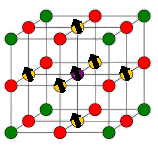
\includegraphics[width=4.5cm,height=4.5cm]{pic/CS.png}
        \end{column}
        % Column 2    
        \begin{column}{0.5\textwidth}
            El Hamiltoniano de intercambio de Heisenberg describe la interacción magnética entre los momentos magnéticos de los electrones en un sistema cuántico.
        \end{column}
    \end{columns}
\end{frame}

\begin{frame}{Energía Magnetostática}
    \begin{columns}
    % Column 1
    \begin{column}{0.5\textwidth}
           \textbf{Energía Zeeman}
           \[ \phi'_H = - \mu_0 \bm{H}_{ext} \cdot \bm{M}_s .\]

            \vspace{0.5cm}
           
           \textbf{Energía dipolar}
           \[ \phi'_s = \frac{\mu_0}{2} \bm{H}_s^2 .\]
           \[\bm{H}_s (\bm{r}) = \frac{1}{4 \pi}  \sum_i \left( \frac{\bm{\mu}_i (\bm{r}_i)}{|\bm{R}|^3} - \frac{3 (\bm{\mu}_i (\bm{r}_i) \cdot \bm{R} ) \cdot \bm{R} }{|\bm{R}|^3}  \right) \]
           \[ \bm{\mu}_i (\bm{r}) = g \mu_B \bm{S}_i (\bm{r}) \]
    \end{column}
    % Column 2    
    \begin{column}{0.5\textwidth}
            \centering
            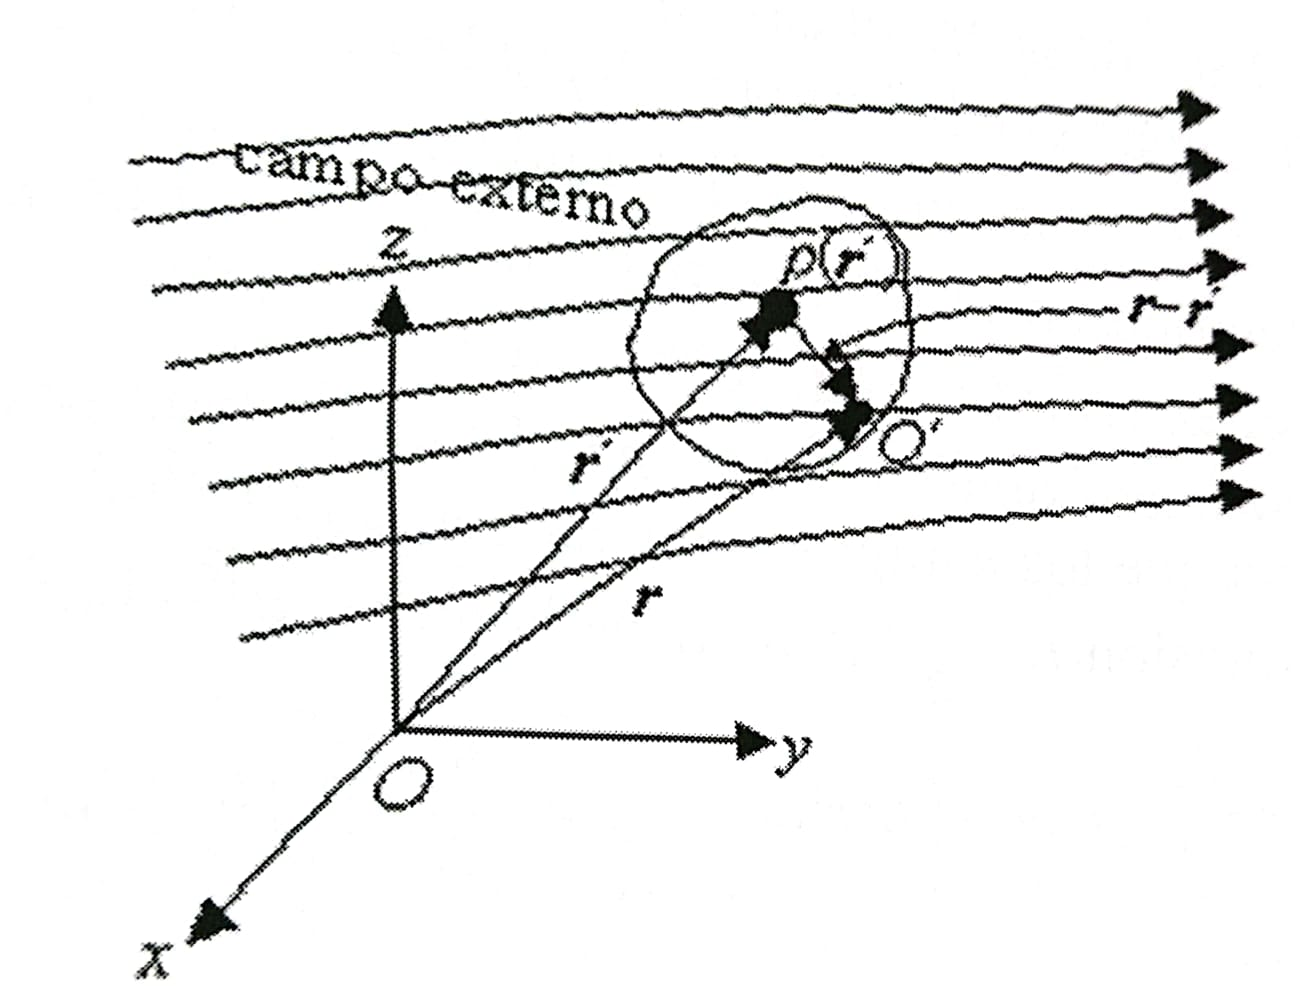
\includegraphics[width=3.5cm,height=3cm]{pic/CampoExterno.jpg}

            \vspace{0.5cm}
            
            \hfill
            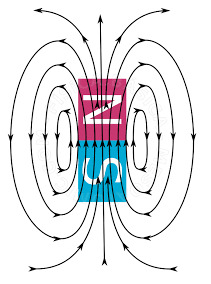
\includegraphics[width=2.5cm,height=3cm]{pic/DipoloMagnetico.png}
    \end{column}
    \end{columns}

\end{frame}

\begin{frame}{Energía de anisotropía magnetocristalina}

%La anisotropia magnetocristalina tiene origen está en la interacción cristal campo y el acoplamiento spin-orbita, o bien las interacción interatomica dipolo-dipolo
    \[ \phi'_K = k_0 (\bm{r}) + \sum_{i \neq j} k_{ij} \gamma_i (\bm{r}) \gamma_j(\bm{r}) + \sum_{ijk} k_{ijk} \gamma_i (\bm{r}) \gamma_j (\bm{r}) \gamma_k (\bm{r}) + \dotsc  \]
    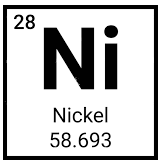
\includegraphics[width=2cm,height=2cm]{pic/Ni.png}
    \hspace{2cm}
    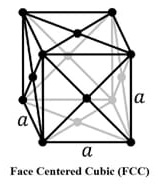
\includegraphics[width=2cm,height=2cm]{pic/Ni-crystal.jpg}
    \hspace{2cm}
    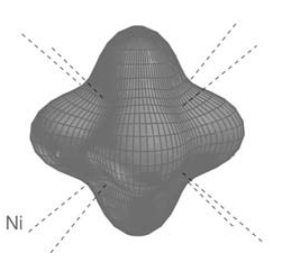
\includegraphics[width=2cm,height=2cm]{pic/Ni-anisotropy.png}

    \vspace{0.5cm}
    
    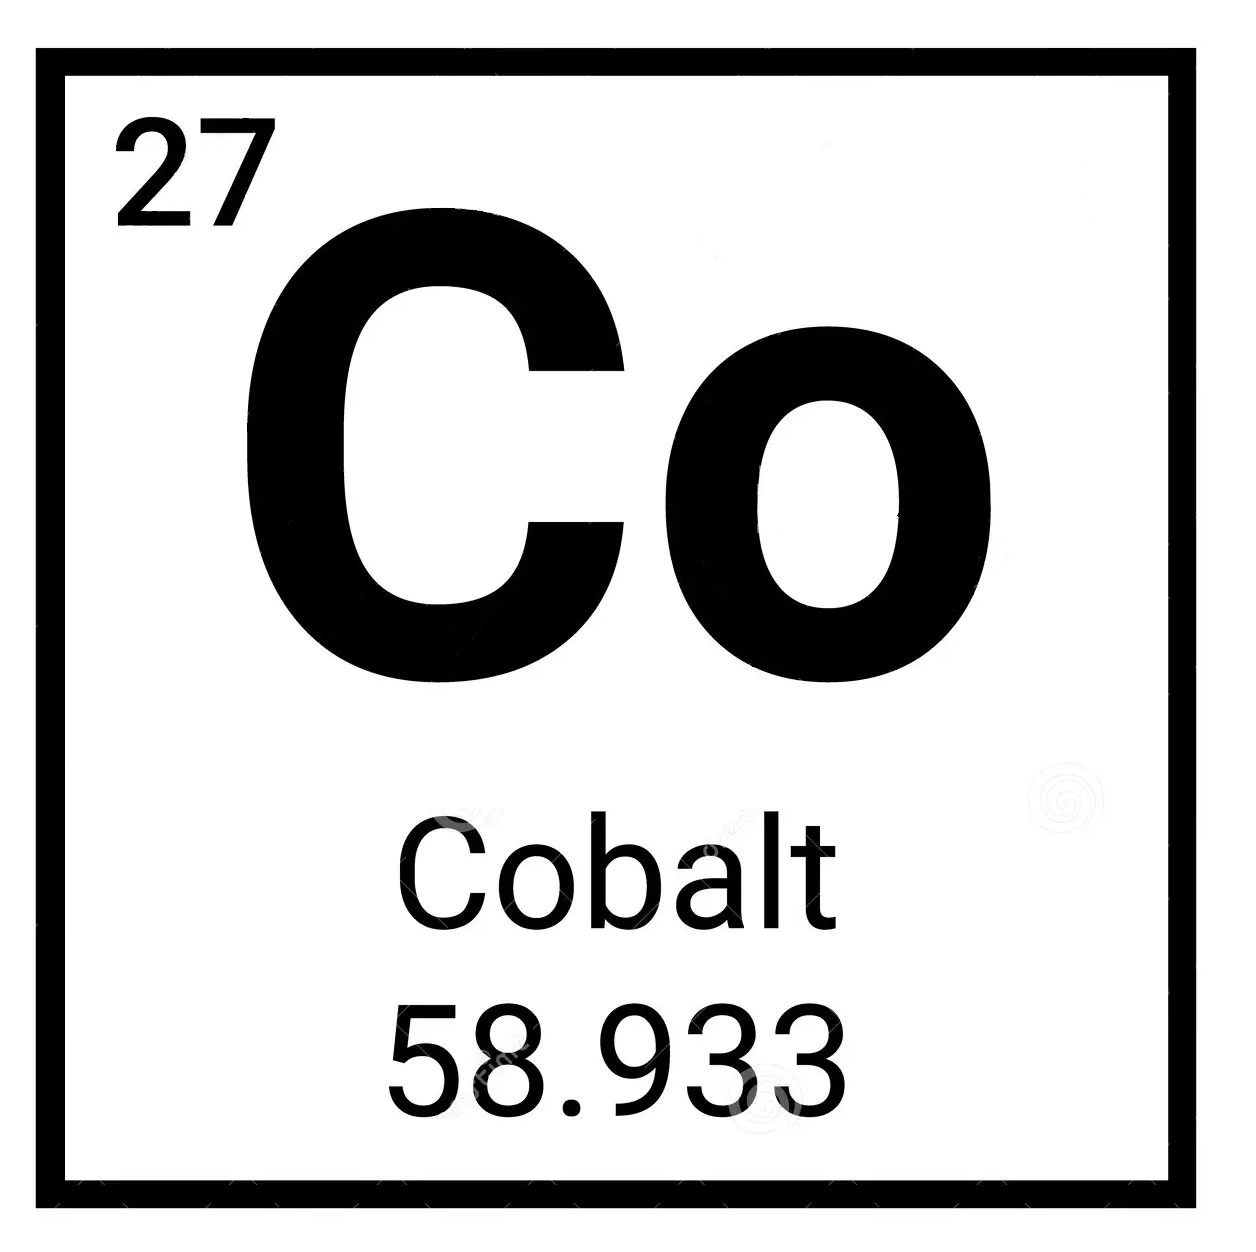
\includegraphics[width=2cm,height=2cm]{pic/Co.png}
    \hspace{2cm}
    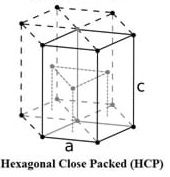
\includegraphics[width=2cm,height=2cm]{pic/Co-crystal.jpg}
    \hspace{2cm}
    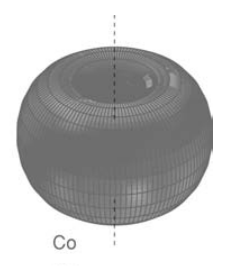
\includegraphics[width=2cm,height=2cm]{pic/Co-anisotropy.png}
    \blfootnote{ {\tiny Coey, J. M. D. Magnetism and Magnetic Materials (Cambridge University Press, 2010).}}
\end{frame}


\begin{frame}{Simulaciones micromagnéticas}
    \begin{columns}
    % Column 1
    \begin{column}{0.5\textwidth}
        \begin{center} 
            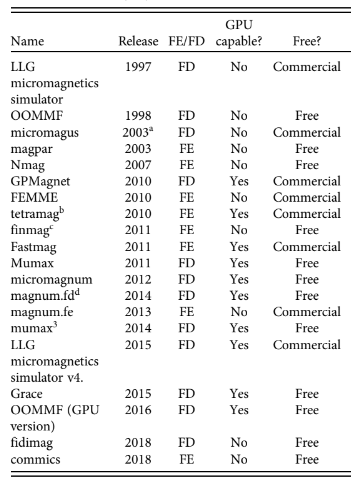
\includegraphics[width=3.8cm,height=4.5cm]{pic/Paquetes.png}
        \end{center}
        \scriptsize
    \textbf{Método numérico}
    \begin{itemize}
        \item \textbf{FD}: Diferencias finitas.
        \item \textbf{FE}: Elementos finitos.
    \end{itemize}
    
    \end{column}
    % Column 2    
    \begin{column}{0.5\textwidth}
    \centering
    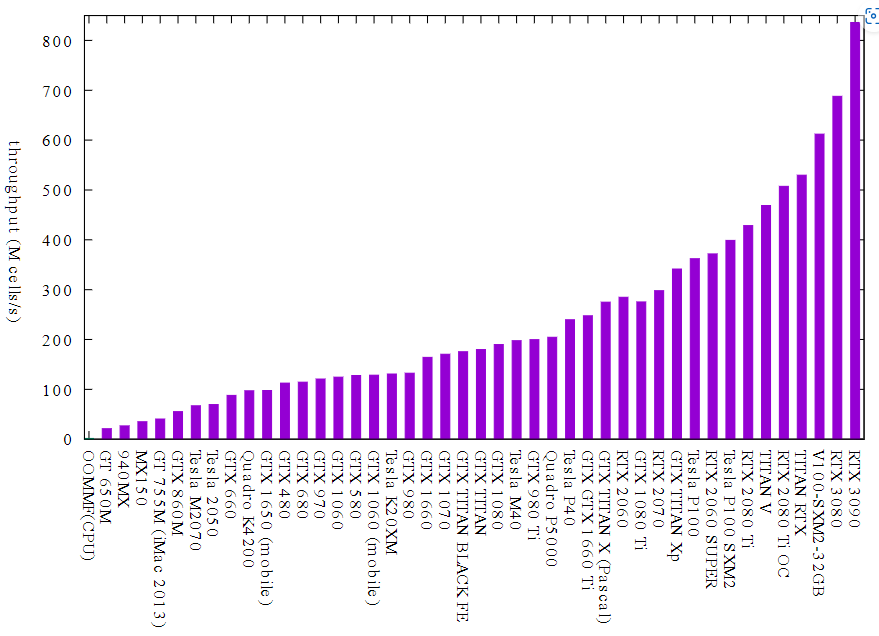
\includegraphics[width=6.5cm,height=4.7cm,angle=90]{pic/GPUs.png}
    \end{column}
    \end{columns}
    \blfootnote{ {\tiny Leliaert, J. Tomorrow's micromagnetic simulations. Journal of Applied Physics 125 (2019). }}
    \blfootnote{ {\tiny https://mumax.github.io/index.html}}
\end{frame}

\section{Objetivos}
\begin{frame}{Objetivos}
    \scriptsize
    \textbf{Objetivo General:}\\
    
    Estudiar la microestructura magnética de nanohilos basados en la aleación Co-Ni y su dependencia con variables intrínsecas y extrínsecas.

    \medskip
    
    \textbf{Objetivos Específicos:}
    \begin{itemize}
        \item Estudiar la dependencia de la microestructura remanente como función de la geometría del nanohilo, la anisotropía magnetocristalina y la composición.

        \item Estudiar el proceso de inversión de la imanación para condiciones y parámetros magnéticos de interés.
    \end{itemize}

    \centering
    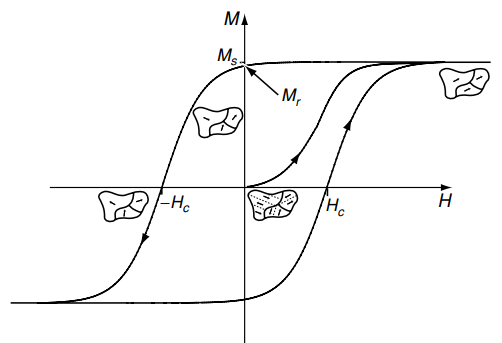
\includegraphics[scale=0.4]{../Figuras/Hysteresis.png}
    
    \blfootnote{{\tiny Coey, J. M. D. Magnetism and Magnetic Materials (Cambridge University Press, 2010).}}
\end{frame}

\section{Metodología}
\begin{frame}{Metodología}
%Esta grafica flue creada usando smartdraw
    \begin{center} 
        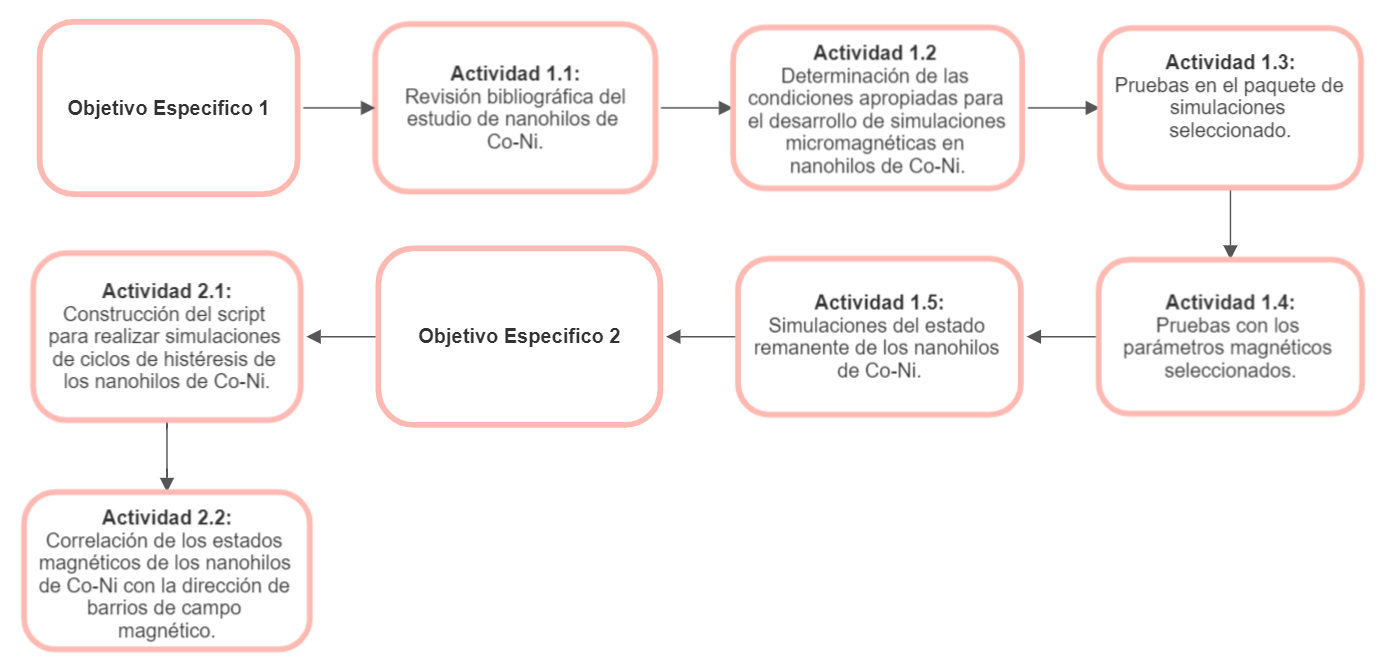
\includegraphics[scale=0.3]{pic/Metodologia.png}
    \end{center}
\end{frame}


\section{Cronograma de Actividades}
\begin{frame}{Cronograma de Actividades}
    \begin{table}[!htp]
        \centering
        \resizebox{11cm}{!}{
            \begin{tabular}{|l|c|c|c|c|c|c|c|c|c|c|c|c|}
                \hline
                & \multicolumn{12}{ |c| }{\textbf{Mes}} \\ \hline
                \multicolumn{1}{|c|}{\textbf{Actividades}} & 01 & 02 & 03 & 04 & 05 & 06 & 07 & 08 & 09 & 10 & 11 & 12 \\ \hline
                \textbf{Actividad 1.1:} Revisión bibliográfica. & x & x & & & & & & & & & & \\ \hline
                \textbf{Actividad 1.2:} Determinación de parámetros micromagnéticos. & & x & x & & & & & & & & & \\ \hline
                \textbf{Actividad 1.3:} Pruebas en el paquete de simulación. & & & x & x & x & & & & & & & \\ \hline
                \textbf{Actividad 1.4:} Pruebas con los parámetros seleccionados. & & & & & x & x & x & x & & & & \\ \hline 
                \textbf{Actividad 1.5:} Simulaciones del sistema. & & & & & & & & x & x & & & \\ \hline
                \textbf{Actividad 2.1:} Script para simular ciclos de histéresis. & & & & & & & & x & x & x & & \\ \hline
                \textbf{Actividad 2.2:} Correlaciones. & & & & & & & & & x & x & x & x \\ \hline
            \end{tabular}
        }
        \caption{Cronograma de actividades}
        \label{tab:Cronograma}
    \end{table}
\end{frame}

\section{Recursos}
\begin{frame}{Recursos}
    \begin{table}[!htp]
        \centering
            \begin{tabular}{|l|c|}
                \hline
                & \textbf{Valor} \\\hline
                Dedicación del asesor: 3 (h/sem) & \$10.600.000 \\ \hline
                Estación de cálculo (Workstation) & \$4.000.000 \\ \hline
                \textbf{Total:} & \$ 14.600.000 \\ \hline
            \end{tabular}
    \end{table}
\end{frame}

\end{document}